\begin{figure}[htb]
    \begin{mdframed}
    \begin{tikzpicture}

        \begin{scope}
            \tikzstyle{box} = [rectangle, rounded corners, minimum width=3.8cm, minimum height=1.6cm,text centered, draw=black, fill=white]

% Population
\node [box] (population) {};
\node [anchor=north] at (population.north) {Population};

\node (line1) [anchor=south west] at (population.south west) {$\coloredrule{10mm}{1mm}{green}$};
\node (line2) [anchor=south west] at (line1.south east) {$\coloredrule{10mm}{1mm}{Salmon}$};
\node (line3) [anchor=south west] at (line2.south east) {$\coloredrule{10mm}{1mm}{Periwinkle}$};
\node (line4) [anchor=south west] at (line1.north west) {$\coloredrule{10mm}{1mm}{red}$};
\node (line5) [anchor=south west] at (line2.north west) {$\coloredrule{10mm}{1mm}{SeaGreen}$};
\node (line6) [anchor=south west] at (line3.north west) {$\coloredrule{10mm}{1mm}{blue}$};
\node (line7) [anchor=south west] at (line4.north west) {$\coloredrule{10mm}{1mm}{Cyan}$};
\node (line8) [anchor=south west] at (line5.north west) {$\coloredrule{10mm}{1mm}{RubineRed}$};
\node (line9) [anchor=south west] at (line6.north west) {$\coloredrule{10mm}{1mm}{OliveGreen}$};

        \end{scope}

        \begin{scope}[xshift=5cm]
            \tikzstyle{box} = [rectangle, rounded corners, minimum width=3.8cm, minimum height=2.1cm,text centered, draw=black, fill=white]

% Phenotypes
\node [box] (phenotypes) {};
\node [anchor=north] at (phenotypes.north) {Phenotypes};
\node (phenotype1) [anchor=south west] at (phenotypes.south west) {\resizebox{0.07\textwidth}{!}{\input{resources/tex/overview/species1.tex}}};
\node (phenotype2) [anchor=south west] at (phenotype1.south east) {\resizebox{0.07\textwidth}{!}{\def\layersep{2.5cm}

\begin{tikzpicture}[shorten >=1pt,->,draw=black!50, node distance=\layersep]
    \tikzstyle{every pin edge}=[<-,shorten <=1pt]
    \tikzstyle{neuron}=[circle,fill=black!25,minimum size=17pt,inner sep=0pt]
    \tikzstyle{input neuron}=[neuron, fill=green!50];
    \tikzstyle{output neuron}=[neuron, fill=red!50];
    \tikzstyle{hidden neuron}=[neuron, fill=blue!50];

    % Draw the input nodes.
    \foreach \name / \y in {1,...,2}
        \node[input neuron] (I-\name) at (0,-\y) {};

    %Draw the hidden node.
    \node[hidden neuron, right of=I-2] (H-1) {};

    % Draw the output node.
    \node[output neuron, right of=H-2] (O-1) {};


    \draw (I-1) -- (O-1) node {};
    \draw (I-2) -- (H-1) node {};
    \draw (H-1) -- (O-1) node {};
    \draw (I-1) -- (H-1) node {};
\end{tikzpicture}}};
\node (phenotype3) [anchor=south west] at (phenotype2.south east) {\resizebox{0.07\textwidth}{!}{\input{resources/tex/overview/species2.tex}}};
\node (phenotype4) [anchor=south west] at (phenotype1.north west) {\resizebox{0.07\textwidth}{!}{\def\layersep{2.5cm}

\begin{tikzpicture}[shorten >=1pt,->,draw=black!50, node distance=\layersep]
    \tikzstyle{every pin edge}=[<-,shorten <=1pt]
    \tikzstyle{neuron}=[circle,fill=black!25,minimum size=17pt,inner sep=0pt]
    \tikzstyle{input neuron}=[neuron, fill=green!50];
    \tikzstyle{output neuron}=[neuron, fill=red!50];
    \tikzstyle{hidden neuron}=[neuron, fill=blue!50];

    % Draw the input nodes.
    \foreach \name / \y in {1,...,2}
        \node[input neuron] (I-\name) at (0,-\y) {};

    %Draw the hidden node.
    \node[hidden neuron, right of=I-2] (H-1) {};

    % Draw the output node.
    \node[output neuron, right of=H-2] (O-1) {};


    \draw (I-1) -- (O-1) node {};
    \draw (I-2) -- (H-1) node {};
    \draw (H-1) -- (O-1) node {};
    \draw (I-1) -- (H-1) node {};
\end{tikzpicture}}};
\node (phenotype5) [anchor=south west] at (phenotype2.north west) {\resizebox{0.07\textwidth}{!}{\input{resources/tex/overview/species1.tex}}};
\node (phenotype6) [anchor=south west] at (phenotype3.north west) {\resizebox{0.07\textwidth}{!}{\input{resources/tex/overview/species2.tex}}};
\node (phenotype7) [anchor=south west] at (phenotype4.north west) {\resizebox{0.07\textwidth}{!}{\input{resources/tex/overview/species2.tex}}};
\node (phenotype8) [anchor=south west] at (phenotype5.north west) {\resizebox{0.07\textwidth}{!}{\def\layersep{2.5cm}

\begin{tikzpicture}[shorten >=1pt,->,draw=black!50, node distance=\layersep]
    \tikzstyle{every pin edge}=[<-,shorten <=1pt]
    \tikzstyle{neuron}=[circle,fill=black!25,minimum size=17pt,inner sep=0pt]
    \tikzstyle{input neuron}=[neuron, fill=green!50];
    \tikzstyle{output neuron}=[neuron, fill=red!50];
    \tikzstyle{hidden neuron}=[neuron, fill=blue!50];

    % Draw the input nodes.
    \foreach \name / \y in {1,...,2}
        \node[input neuron] (I-\name) at (0,-\y) {};

    %Draw the hidden node.
    \node[hidden neuron, right of=I-2] (H-1) {};

    % Draw the output node.
    \node[output neuron, right of=H-2] (O-1) {};


    \draw (I-1) -- (O-1) node {};
    \draw (I-2) -- (H-1) node {};
    \draw (H-1) -- (O-1) node {};
    \draw (I-1) -- (H-1) node {};
\end{tikzpicture}}};
\node (phenotype9) [anchor=south west] at (phenotype6.north west) {\resizebox{0.07\textwidth}{!}{\input{resources/tex/overview/species1.tex}}};

        \end{scope}

        \begin{scope}[xshift=7.7cm, yshift=-2.4cm, scale=0.8, every node/.append style={transform shape}]
            \tikzstyle{box} = [rectangle, rounded corners, minimum width=2.5cm, minimum height=1.2cm,text centered, draw=black]

\node [box] (agent) {};
\node [anchor=north] at (agent.north) {Agent};

\node (network) [anchor=south] at (agent.south) {\resizebox{0.15\textwidth}{!}{\def\layersep{2.5cm}

\begin{tikzpicture}[shorten >=1pt,->,draw=black!50, node distance=\layersep]
    \tikzstyle{every pin edge}=[<-,shorten <=1pt]
    \tikzstyle{neuron}=[circle,fill=black!25,minimum size=17pt,inner sep=0pt]
    \tikzstyle{input neuron}=[neuron, fill=green!50];
    \tikzstyle{output neuron}=[neuron, fill=red!50];
    \tikzstyle{hidden neuron}=[neuron, fill=blue!50];

    % Draw the input nodes.
    \foreach \name / \y in {1,...,2}
        \node[input neuron] (I-\name) at (0,-\y) {};

    %Draw the hidden node.
    \node[hidden neuron, right of=I-2] (H-1) {};

    % Draw the output node.
    \node[output neuron, right of=H-2] (O-1) {};


    \draw (I-1) -- (O-1) node {};
    \draw (I-2) -- (H-1) node {};
    \draw (H-1) -- (O-1) node {};
    \draw (I-1) -- (H-1) node {};
\end{tikzpicture}}};

\tikzstyle{box} = [rectangle, rounded corners, minimum width=2.5cm, minimum height=0.8cm,text centered, draw=black]
\node [box, right=1.4cm of agent] (environment) {Environment};
\tikzstyle{arrow} = [thick,->,>=stealth]
%\draw[-latex, thick] (agent) -- (agent-|environment.west) node[midway, below, text width=1cm]{action};
\draw [arrow] (environment.north) --++(0,0.1) |- (agent.north);

%\draw[-latex, thick] (environment.north) -- (environment.north-|agent.north) node[midway, above, text width=1cm]{reward};

        \end{scope}

        \begin{scope}[xshift=10cm, yshift=-5cm]
            
\node [box] (speciate) {};
\node [anchor=north] at (speciate.north) {Speciation};

\node (line1) [anchor=south west] at (speciate.south west) {$\coloredrule{10mm}{1mm}{OliveGreen}$};
\node (line2) [anchor=south west] at (line1.south east) {$\coloredrule{10mm}{1mm}{RubineRed}$};
\node (line3) [anchor=south west] at (line2.south east) {$\coloredrule{10mm}{1mm}{blue}$};
\node (line4) [anchor=south west] at (line1.north west) {$\coloredrule{10mm}{1mm}{green}$};
\node (line5) [anchor=south west] at (line2.north west) {$\coloredrule{10mm}{1mm}{red}$};
\node (line6) [anchor=south west] at (line3.north west) {$\coloredrule{10mm}{1mm}{Periwinkle}$};
\node (line7) [anchor=south west] at (line4.north west) {$\coloredrule{10mm}{1mm}{SeaGreen}$};
\node (line8) [anchor=south west] at (line5.north west) {$\coloredrule{10mm}{1mm}{Salmon}$};
\node (line9) [anchor=south west] at (line6.north west) {$\coloredrule{10mm}{1mm}{Cyan}$};


        \end{scope}

        \begin{scope}[xshift=5cm, yshift=-5cm]
            
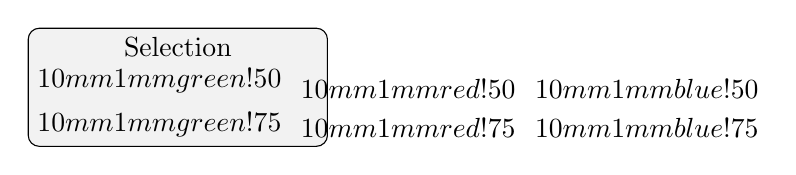
\begin{tikzpicture}
    \tikzstyle{box} = [rectangle, rounded corners, minimum width=3.8cm, minimum height=1.5cm,text centered, draw=black, fill=gray!10]

    \node [box] (selection) {};
    \node [anchor=north] at (selection.north) {Selection};

    \node (line1) [anchor=south west] at (selection.south west) {$\coloredrule{10mm}{1mm}{green!75}$};
    \node (line2) [anchor=south west] at (line1.south east) {$\coloredrule{10mm}{1mm}{red!75}$};
    \node (line3) [anchor=south west] at (line2.south east) {$\coloredrule{10mm}{1mm}{blue!75}$};
    \node (line4) [anchor=south west] at (line1.north west) {$\coloredrule{10mm}{1mm}{green!50}$};
    \node (line5) [anchor=south west] at (line2.north west) {$\coloredrule{10mm}{1mm}{red!50}$};
    \node (line6) [anchor=south west] at (line3.north west) {$\coloredrule{10mm}{1mm}{blue!50}$};

  \end{tikzpicture}
        \end{scope}

        \begin{scope}[xshift=0cm, yshift=-5cm]
            

\node [box] (reproduction) {};
\node [anchor=north] at (reproduction.north) {Reproduction};

\node (line1) [anchor=south west] at (reproduction.south west) {$\coloredrule{10mm}{1mm}{OliveGreen, green}$};
\node (line2) [anchor=south west] at (line1.south east) {$\coloredrule{10mm}{1mm}{red, Salmon}$};
\node (line3) [anchor=south west] at (line2.south east) {$\coloredrule{10mm}{1mm}{blue, Periwinkle}$};
\node (line4) [anchor=south west] at (line1.north west) {$\coloredrule{10mm}{1mm}{green, OliveGreen}$};
\node (line5) [anchor=south west] at (line2.north west) {$\coloredrule{10mm}{1mm}{Salmon, red}$};
\node (line6) [anchor=south west] at (line3.north west) {$\coloredrule{10mm}{1mm}{Periwinkle, blue}$};
\node (line7) [anchor=south west] at (line4.north west) {$\coloredrule{10mm}{1mm}{green}$};
\node (line8) [anchor=south west] at (line5.north west) {$\coloredrule{10mm}{1mm}{red}$};
\node (line9) [anchor=south west] at (line6.north west) {$\coloredrule{10mm}{1mm}{blue}$};
        \end{scope}

        \begin{scope}[xshift=0cm, yshift=-2.5cm]
            
  \node [box] (mutation) {};
  \node [anchor=north] at (mutation.north) {Mutation};

  % TODO: slightly shift the color of the offspring.


  \node (line1) [anchor=south west] at (mutation.south west) {$\coloredrule{10mm}{1mm}{green!75}$};
  \node (line2) [anchor=south west] at (line1.south east) {$\coloredrule{10mm}{1mm}{red!75}$};
  \node (line3) [anchor=south west] at (line2.south east) {$\coloredrule{10mm}{1mm}{blue!75}$};
  \node (line4) [anchor=south west] at (line1.north west) {$\coloredrule{10mm}{1mm}{green!50}$};
  \node (line5) [anchor=south west] at (line2.north west) {$\coloredrule{10mm}{1mm}{red!50}$};
  \node (line6) [anchor=south west] at (line3.north west) {$\coloredrule{10mm}{1mm}{blue!50}$};

        \end{scope}

    \end{tikzpicture}
    \end{mdframed}
\end{figure}